\documentclass[a4paper,12pt,fleqn]{article}%fleqn pour aligner les equations à gauche
\usepackage{../../Styles/Cours}


\newcommand{\chnum}{Chapitre 11}
\newcommand{\chtitle}{Explorer les champs}
\newcommand{\dtype}{TP}

\begin{document}
	\maketitle
\begin{figure}[h!]
    \caption{Un champ ?}
    \label{doc1}
    Un objet, de par ses propriétés physiques (masse, charge, ...) modifie les propriétés de l'espace qui l'entoure. On dit alors qu'il crée un champ autour de lui. Des objets ayant les mêmes propriétés physiques, subissent alors une force lorsqu'ils sont placés sur ce champ.\\
    Le champ électrostatique $\vv{E}$ caractérise l'influence qu'une charge électrique peut exercer que une autre charge. La force électrostatique subie par la charge $q$ placée dans ce champ est telle que : $\vv{F} = q \cdot \vv{E}$.
\end{figure}
\begin{figure}[h!]
    \caption{influence d'un champ électrostatique}
    \label{doc2}
    \begin{minipage}{.49\linewidth}
        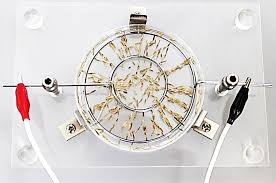
\includegraphics[height=5cm]{Ressources/1SPE_C11_AE2_PointeRheo.png}\\
        \centering Des graines dans une cuve chargée
    \end{minipage}
    \begin{minipage}{.49\linewidth}
        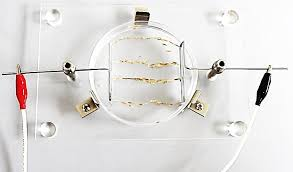
\includegraphics[height=5cm]{Ressources/1SPE_C11_AE2_PlaqueRheo.png}\\
        \centering Des graines dans une cuve entre deux plaques chargées positivement et négativement
    \end{minipage}
\end{figure}

\begin{figure}[h!]
    \caption{Définitions}
    \label{doc3}
    Le vecteur champ électrostatique $\vv{E}$ est toujours orienté du positif vers le négatif. Son unité est le volt par mètre (\unit{\volt\per\meter}).\\
    Les lignes de champ électrostatique sont des courbes tangentes au vecteur champ. Elles sont orientées par une flèche dans le même sens que celui du champ.\\
    Cartographier un champ électrostatique consiste à tracer les lignes de champ dans une zone donnée.\\
    Èquipotentielle : une surface équipotentielle d'un champ électrique est l'ensemble des points où la tension électrique est la même.
\end{figure}

\begin{figure}[h!]
    \caption{Cartographier un champ}
    \label{doc4}
    \begin{minipage}{.35\linewidth}
        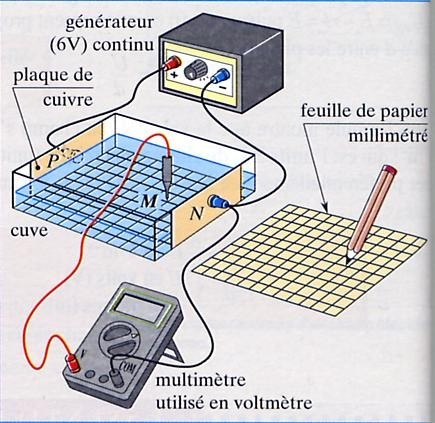
\includegraphics[width=\linewidth]{Ressources/1SPE_C11_AE2_Montage.png}
    \end{minipage}
    \begin{minipage}{.65\linewidth}
        La cuve "rhéologique" est un dispositif qui permet de cartographier le champ électrosstatique existant entre deux électrodees conductrices "chargées". Elle est constituée d'une cuve au fond de laquelle un repère quadrillé est immergé dans une faible épaisseur (environ \SI{1}{cm}) de solution conductrice de sulfate de cuivre. Des plaques de cuivre trempent dans la solution conducteice et sont reliées à une source de tension continue (ici ce 6V).\\
    La tension électrique exprime la différence de potentiel électrique entre deux points d'un circuit. on l'exprime en \unit{\volt} et on la mesure à l'aide d'un voltmètre.\\
    \textit{Exemple : entre les points $M$ et $N$, on a : $U_{MN} = V_M-V_N$.}\\
    Si l'on choisit un potentiel nul en un point relié à la borne COM du voltmètre, la tension affichée sera égale au potentiel du point électrique du point $M$.\\
    \end{minipage}
\end{figure}

\begin{enumerate}
    \item Quelles entités conduisent le courant dans la solution de sulfate de cuivre ?
    \item Déplacer la sonde sur la plaque $P$, reliée à la borne + du générateur. Faire de même sur la plaque $N$. Noter les tensions mesurées sur chacune des plaques. Compléter : $$ U_P = \text{...... V}$$
    \item Peut-on dire que chaque plaque constitue un équipotentiel ? Justifier.
    \item Déplacer la sonde sur la ligne perpendiculaire de la plaque $N$, en allant de $N$ vers $P$. Noter vos observations.
    \item Déplacer la sonde sur une ligne parallèle aux plaques, dans la cuve. Noter vos observations.
    \item Repérer dans la cuve les endroits qui vérifient $U_{MN} = \SI{3,0}{V}$. Faire une description de l'endroit trouvé.
    \item Sur le schéma fourni, noter le nom des plaques puis tracer des équipotentielles en vert.
    \item Sachant que les lignes de champ sont partout perpendiculaires aux équipotentielles, représenter en bleu, l'allure des lignes de champ entre les plaques métalliques.
    \item Orienter avec une petite flèche les lignes de champ. Justifier cette orientation.
    \item La valeur du champ électrostatique $E$ entre les armatures se détermine, en tout point $M$ par la relation : $$ E = \dfrac{U}{d}$$ où $U$ est la tension entre les armatures et $d$ la distance entre celles-ci. Compléter le tableau de mesure en utilisant la cuve rhéographique.
    \item Commenter la valeur du champ électrostatique relevés.
    \item Traver le vecteur champ en plusieurs points sur le schéma fourni
\end{enumerate}

\begin{table}
    \centering
    \begin{tabular}{|>{\centering}m{.3\linewidth}|>{\centering}m{.3\linewidth}|>{\centering\arraybackslash}m{.3\linewidth}|}
        \hline
        \textbf{Tension électrique $U_{MN}$} & \textbf{Distance $MN$ correspondante} & \textbf{Calcul $\dfrac{U_{MN}}{MN}$} \\
        \hline
        \SI{3,0}{V} & & \\
        \hline
        \SI{4,0}{V} & & \\
        \hline
        \SI{5,0}{V} & & \\
        \hline
    \end{tabular}
\end{table}

\newpage
\begin{figure}
    \centering
    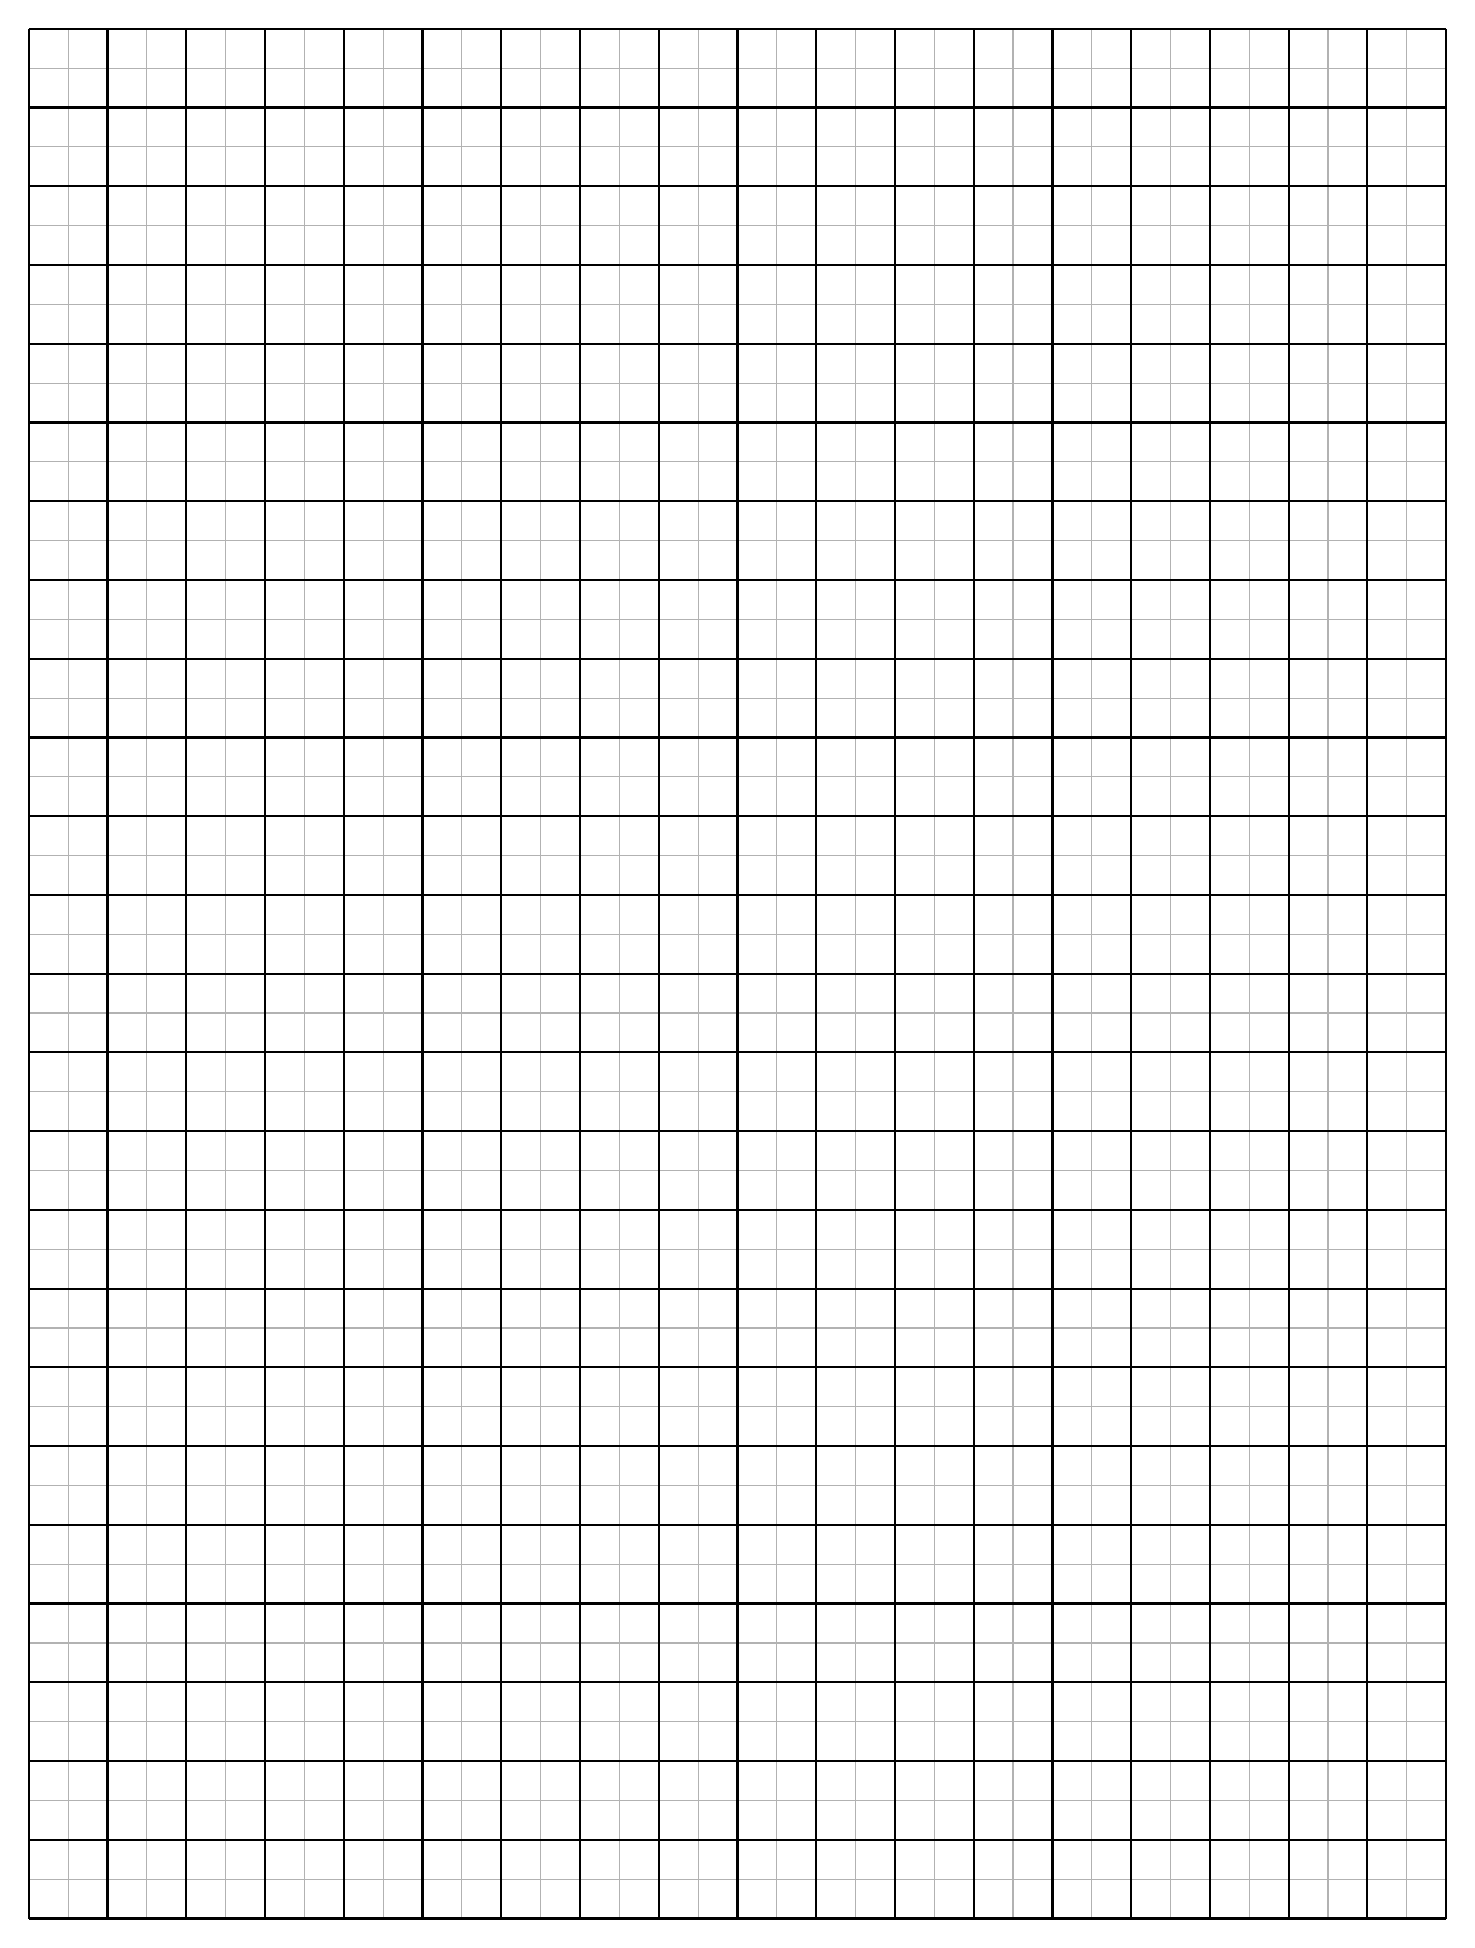
\begin{tikzpicture}
    \draw[gray!60] (0,0) grid[step = .5](18,24);
    \draw[thick] (0,0) grid(18,24);
    
    \end{tikzpicture}
\end{figure}
\end{document}